\documentclass[10pt]{jarticle}

\usepackage{amssymb,color,amsmath,dcolumn,array,graphicx,amsthm}
\newtheorem{Def}{定義}[section]
\newtheorem{Prp}{命題}[section]
\newtheorem{Lem}{補題}[section]
\renewcommand \proofname{\bf 証明}
\newcommand{\exprx}{e^{[\boldsymbol{r}]_{\times}}}
\newcommand{\rx}{[\boldsymbol{r}]_{\times}}
\newcommand{\brx}{[\bar{\boldsymbol{r}}]_{\times}}

\begin{document}

\title{Euclid変換\\~3次元空間の回転と並進を中心として~}
\author{小川 雅弘}
\date{\today}
\maketitle

\tableofcontents

\section{序論}
この記事では、回転と並進で表わされる、Euclid変換についてまとめる。

\subsection{記号の定義}
\begin{itemize}
\item 各点の位置ベクトルは点の記号を太字で書く。例)$\boldsymbol{x}$ 
\item ベクトルの各座標系での表示をベクトルの右下に/\{座標系\} で表示する。
例)$\boldsymbol{x}_{/A}$:ベクトル$\boldsymbol{x}$のA座標系での表示 
\item ベクトルの、各座標系での表示の転置は、左上添え字にtをつける。例)$^t\boldsymbol{x}_{/A}$
\item 座標系$\mathcal{O}_i$の原点は、$\boldsymbol{o}_i$ と表す。 
\item $\mathcal{O}\{ x,y,z \} $: 原点を$\boldsymbol{o}_i$、x,y,z軸を右手系とした直交直線座標系。
\item $\bar{\boldsymbol{x}}$: ベクトル$\boldsymbol{x}$の、長さを1に正規化したベクトル
\item $E_n$: n次の単位行列
\item $O_n$: n次のゼロ行列
\item $\det(A)$: 行列Aのdeterminant
\item $\mathrm{Tr}(A)$: 行列Aのtrace
\item $M(n,\mathbb{R})$: 実数を成分とするn次正方行列の集合
\item $GL(n,\mathbb{R}):=\{A \in M(n,\mathbb{R}) | Aは正則\}$
\item $SO(n):=\{A \in M(n,\mathbb{R}) | {}^tAA=E_n, \det(A)=1 \}$
\item $U(n):=\{A \in M(n,\mathbb{C}) | A^*A=E_n\}$
\item $R(\boldsymbol{r},\theta)$: 回転軸$\boldsymbol{r}$、回転量$\theta$の回転行列
\item $(A_{ij})$: ij成分が$A_{ij}$の行列
\end{itemize}



\section{一般のEuclid変換}
対象点$\boldsymbol{x}$の、座標系$\mathcal{O}_1$から座標系$\mathcal{O}_2$へのEuclid座標変換(回転+並進)は下記のように表わされる。
\begin{eqnarray}
\boldsymbol x_{/\mathcal{O}_2} 
&=& R_{\mathcal O_1\rightarrow \mathcal O_2} \boldsymbol x_{/\mathcal O_1} + \boldsymbol t_{\mathcal O_1\rightarrow \mathcal O_2 /\mathcal O_2} \\
&=& R(\theta_{\mathcal O_2\rightarrow \mathcal O_1}) \boldsymbol x_{/\mathcal O_1} + \overrightarrow{o_2 o_1}_{/\mathcal O_2}\label{eq:EucTr}
\end{eqnarray}
ここで、$\theta_{\mathcal O_1\rightarrow \mathcal O_2}$は、座標系$\mathcal{O}_1$を座標系$\mathcal{O}_2$へ重ねる回転角度を表し、
$\overrightarrow{o_1 o_2}$は、$\boldsymbol{o}_1$から$\boldsymbol{o}_2$へ向かうベクトル表す。

具体的な形については、次元ごとに次節以降で扱う。



\section{2次元Euclid変換}
\subsection{公式}
一般の場合の(\ref{eq:EucTr})式がそのまま適用でき、
\begin{eqnarray}
\boldsymbol x_{/\mathcal{O}_2} 
= R(\theta_{\mathcal O_2\rightarrow \mathcal O_1}) \boldsymbol x_{/\mathcal O_1} + \overrightarrow{o_2 o_1}_{/\mathcal O_2}
\label{eq:2dEucTr}
\end{eqnarray}
となる。


\subsection{具体例}
本節では、具体的な座標変換で、座標変換公式(\ref{eq:2dEucTr})を確認する。

2次元Euclid変換の自由度は、回転1、並進2の3自由度ある。
1点は2つの独立な条件を定めるので、(\ref{eq:2dEucTr})の確認のためには、
異なる2点が正しく変換されていることを見れば十分である。

\begin{itemize}
\item 例1) 並進
  \begin{figure}[htb]
    \centering
    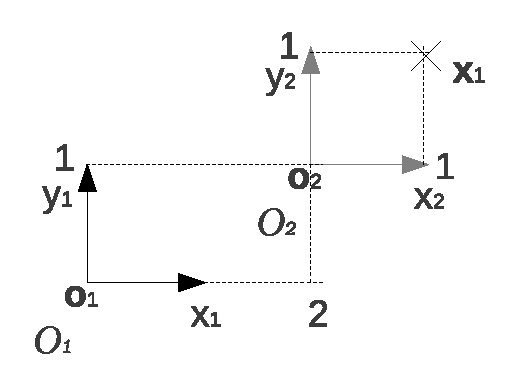
\includegraphics[width=3cm]{ex1.eps}
    \caption{例1の見取り図}
    \label{fig:ex1}
  \end{figure}
\begin{eqnarray}
\boldsymbol{x}_{/\mathcal{O}_2} = \boldsymbol x_{/\mathcal O_1} - {}^t(2,1)
\end{eqnarray}
確認は2点で十分だが、念のため、確認用の点として、
$\boldsymbol{o}_1, \boldsymbol{o}_2, \boldsymbol{x}_{1/\mathcal O_1}= {}^t(3,2)$
の3点をとると、
\begin{eqnarray}
\boldsymbol{o}_{1/\mathcal O_1} - {}^t(2,1) = {}^t(0,0)-{}^t(2,1) = -{}^t(2,1) = \boldsymbol{o}_{1/\mathcal{O}_2} \nonumber\\
\boldsymbol{o}_{2/\mathcal O_1} - {}^t(2,1) = {}^t(2,1)-{}^t(2,1) = {}^t(0,0) = \boldsymbol{o}_{2/\mathcal{O}_2} \nonumber\\
\boldsymbol{x}_{1/\mathcal O_1} - {}^t(2,1) = {}^t(3,2)-{}^t(2,1) = {}^t(1,1) = \boldsymbol{x}_{1/\mathcal{O}_2} \nonumber
\end{eqnarray}
となり、(\ref{eq:2dEucTr})式の正しさが確認できる。

\item 例2) 回転と並進
  \begin{figure}[htb]
    \centering
    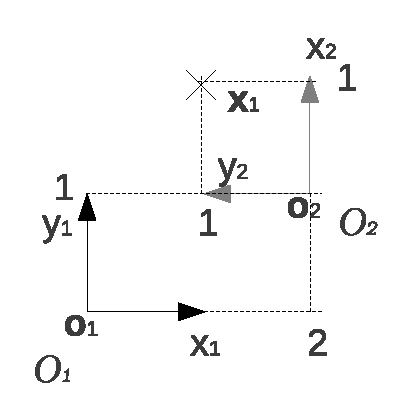
\includegraphics[width=3cm]{ex2.eps}
    \caption{例2の見取り図}
    \label{fig:ex2}
  \end{figure}
\begin{eqnarray}
\boldsymbol{x}_{/\mathcal{O}_2} = R \boldsymbol x_{/\mathcal O_1} + {}^t(-1,2)\\
R=\left(
\begin{array}{ccc}
0 &1  \\
-1& 0
\end{array}
\right)
\end{eqnarray}
確認用の点として、$\boldsymbol{o}_1, \boldsymbol{o}_2, \boldsymbol{x}_{1/\mathcal O_1}={}^t(1,2)$
の3点をとると、
\begin{eqnarray}
R \boldsymbol{o}_{1/\mathcal O_1} + {}^t(-1,2) = R{} ^t(0,0) + {}^t(-1,2) = ^t(-1,2) = \boldsymbol{o}_{1/\mathcal{O}_2} \nonumber\\
R \boldsymbol{o}_{2/\mathcal O_1} + {}^t(-1,2) = R\ ^t(2,1) + ^t(-1,2) =^t(0,0) = \boldsymbol{o}_{2/\mathcal{O}_2} \nonumber\\
R \boldsymbol{x}_{1/\mathcal O_1} + {}^t(-1,2) = R\ ^t(1,2) + ^t(-1,2) =^t(1,1) = \boldsymbol{x}_{1/\mathcal{O}_2} \nonumber
\end{eqnarray}
となり、(\ref{eq:2dEucTr})式の正しさが確認できる。
\end{itemize}



\section{3次元Euclid変換}
3次元Euclid変換も、(\ref{eq:EucTr})で表され、並進についてはこの表現で定まるが、
回転についてはいくつかの表示がありうる。
そこで本章では、3次元空間の回転($R_{\mathcal O_1\rightarrow \mathcal O_2}$)について扱っていく。
\subsection{行列による回転の表現}
\subsubsection{基底による回転行列の表現}
回転は、座標系$\mathcal{O}_1、\mathcal{O}_2$の基底ベクトルをそれぞれ、
$\boldsymbol {e_{1x},e_{1y},e_{1z}}、\boldsymbol {e_{2x},e_{2y},e_{2z}}$
とすると、

\begin{eqnarray}
R_{\mathcal O1\rightarrow \mathcal O2} =
\left[ 
\begin{array}{ccc}
^t \boldsymbol  e_{2x/\mathcal O1} \\
^t \boldsymbol  e_{2y/\mathcal O1} \\
^t \boldsymbol  e_{2z/\mathcal O1} \\
\end{array} 
\right]
\end{eqnarray} 

これは、$R,\boldsymbol  t$ は合計6自由度なので、2本の独立なベクトルの変換が正しくできていることを確かめれば、
6個の拘束条件がつくため十分であり、2本のベクトルとして、
$\boldsymbol  {e_{2x},e_{2y}}$ を、式(\ref{eq:EucTr})の$\boldsymbol  x_{/O1}$に代入すれば確かめられる。

\subsubsection{roll, pitch, yawによる回転行列の表現}
X,Y,Z各軸の正方向を軸とした、右ねじ方向への回転角をそれぞれ、roll, pitch, yawと呼ぶ。
座標系$\mathcal{O}_2$を、座標系$\mathcal{O}_2$でのyaw, pitch, rollの順に回転すると、座標系$\mathcal{O}_1$に重なるとする。
これを、Tate-Bryantの分解という。
これを図で表したものが、図\ref{trans}である。
\begin{figure}[htb]
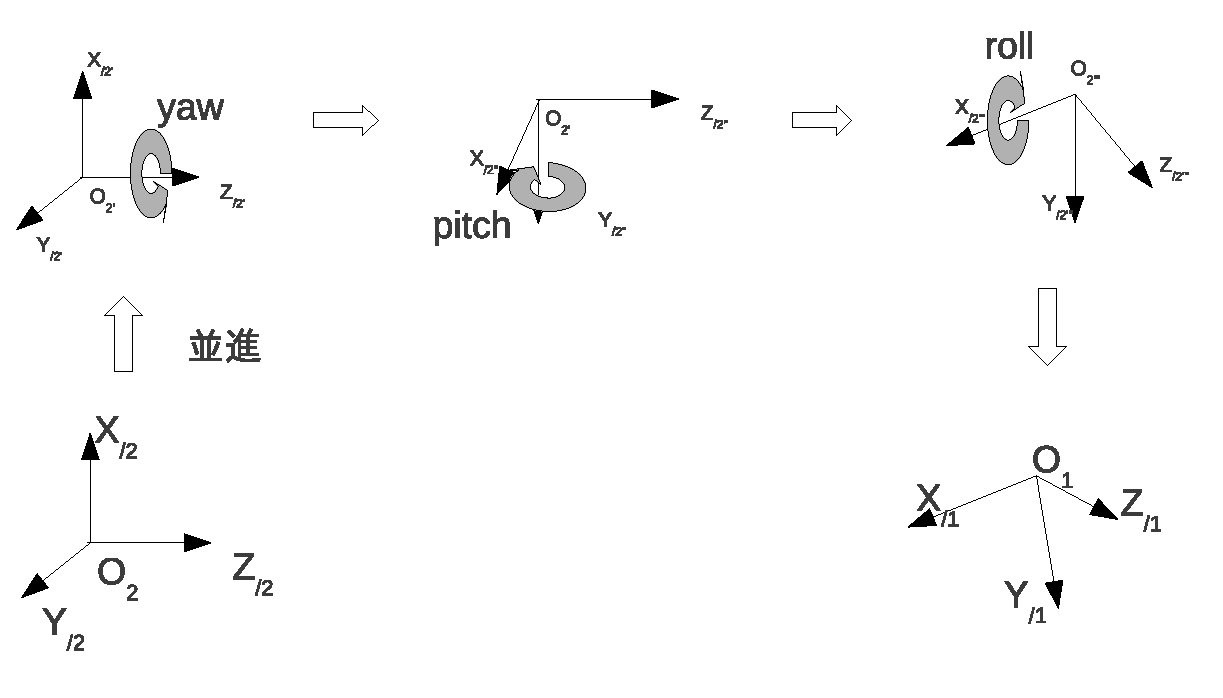
\includegraphics[width = 13cm]{EuclidTransformation.eps}
\caption{Euclid transformation from O1 to O2}
\label{trans}
\end{figure}

今、
\begin{eqnarray}
    R(roll):=\left(
      \begin{array}{ccc}
          1&0&0\\
          0&\cos(roll)&-\sin(roll)\\
          0&\sin(roll)&\cos(roll)
      \end{array}
      \right)\\
    R(pitch):=\left(
      \begin{array}{ccc}
          \cos(pitch)&0&\sin(pitch)\\
          0&1&0\\
          -\sin(pitch)&0&\cos(pitch)
      \end{array}
      \right)\\
    R(yaw):=\left(
      \begin{array}{ccc}
          \cos(yaw)&-\sin(yaw)&0\\
          \sin(yaw)&\cos(yaw)&0\\
          0&0&1
      \end{array}
    \right)
\end{eqnarray}
としたとき、回転行列は、このroll, pitch, yawの組み合わせで、下記のように表わされる。(分かり易さのため、並進も併せて表す。)
\begin{eqnarray}
\boldsymbol x_{/\mathcal{O}_1} &=& R(-roll) R(-pitch) R(-yaw) (\boldsymbol x_{/\mathcal O_2} - \overrightarrow{o_2 o_1}_{/\mathcal O_2})\\
\Rightarrow
\boldsymbol x_{/\mathcal{O}_2} &=& R(yaw) R(pitch) R(roll) \boldsymbol x_{/\mathcal O_1} + \overrightarrow{o_2 o_1}_{/\mathcal O_2}\\
\Rightarrow
R_{\mathcal O1\rightarrow \mathcal O2} &=& R(yaw) R(pitch) R(roll)
\end{eqnarray}


\subsection{ベクトルによる回転の表現}
回転は、回転軸中心と、その軸周りの回転量でも表わされる。\\
回転ベクトル$\boldsymbol{r}$を、向き$\frac{\boldsymbol{r}}{||\boldsymbol{r}||}=\boldsymbol{\bar{r}}$が回転軸方向で、
大きさ$||\boldsymbol{r}||=:\theta$が、回転量を表すベクトルとして定義する。
以下では、この$\boldsymbol{r}$と回転行列の関係を調べる。

\subsubsection{回転ベクトルからの回転行列の作成}
まず、$\boldsymbol{r}$から回転行列を作る。
\begin{Def}
    \begin{eqnarray}
        \boldsymbol{r}_{/\mathcal{O}} = {}^t(r_1,r_2,r_3)\\
        {[\boldsymbol{r}]_{\times}} := 
        \left(
          \begin{array}{ccc}
              0 &-r_3 &r_2  \\
              r_3 & 0& -r_1 \\
              -r_2 & r_1& 0
          \end{array}
        \right) \\
        e^{[\boldsymbol{r}]_{\times}}:=\sum_{n=0}^{\infty}\frac{[\boldsymbol{r}]_{\times}{}^n}{n!} \label{eq:defe^r}
    \end{eqnarray}
\end{Def}

と定義したとき、次の命題が成り立つ。

\begin{Prp}\label{thm:rotvec}
    $e^{[\boldsymbol{r}]_{\times}}$は回転行列であり、その回転軸は$\boldsymbol{r}$、回転角度は$||\boldsymbol{r}||$である。
\end{Prp}


つまりこの命題によれば、回転ベクトル$\boldsymbol{r}$が分かっているとき、$e^{[\boldsymbol{r}]_{\times}}$が、
$\boldsymbol{r}$に対応する回転行列になる、ということである。
命題\ref{thm:rotvec}を証明するため、以下の補題を示す。

\begin{Lem} \label{lem:powerOfE}
    $A,B \in M_3(\mathbb{R}) \ s.t.$(such that)  $AB=BA$
    に対し、
    \begin{equation}
        e^A e^B = e^B e^A = e^{A+B}
    \end{equation}
\end{Lem}

\begin{proof}
    \begin{eqnarray}
        e^{A+B}&=&\sum_{n=0}^{\infty} \frac{(A+B)^n}{n!}\nonumber\\
        &=&\sum_{n=0}^{\infty}\frac{1}{n!} \sum_{m=0}^n {}_nC_m A^m B^{n-m} \hspace{5mm}(\because AB=BA) \nonumber\\
        &=&\sum_{n=0}^{\infty}\sum_{m=0}^n \frac{A^m B^{n-m}}{m! (n-m)!} \nonumber\\
        &=&(E_3+\frac{B}{1!}+\frac{B^2}{2!}+\hdots)+\frac{A}{1!}(E_3+\frac{B}{1!}+\frac{B^2}{2!}+\hdots) \nonumber\\
        &&+\frac{A^2}{2!}(E_3+\frac{B}{1!}+\frac{B^2}{2!}+\hdots)+\hdots \nonumber\\
        &=&(\sum_{n=0}^{\infty} \frac{A^n}{n!}) (\sum_{m=0}^{\infty} \frac{B^m}{m!}) \nonumber\\
        &=&e^A e^B = e^B e^A \nonumber
    \end{eqnarray}
\end{proof}

\begin{Lem} \label{lem:detTr}
    $A \in M_3(\mathbb{R})$に対し、
    \begin{equation}
        \det(e^A) = e^{\mathrm{Tr}(A)}
    \end{equation}
\end{Lem}

\begin{proof}
    \begin{eqnarray}
        \exists P\in GL(3,\mathbb{R})&&  s.t. \ 
        P^{-1}AP=
        \left(
          \begin{array}{ccc}
              \lambda_1 & * & * \\
              0 & \lambda_2 & * \\
              0 & 0 & \lambda_3
          \end{array}
        \right) \nonumber\\
        \det(e^A)&=&\det(P^{-1}e^AP) \nonumber\\
        &=&\det(e^{P^{-1}AP}) \nonumber\\
        &=&\det(\sum_{n=0}^{\infty}\frac{1}{n!}
        \left(
          \begin{array}{ccc}
              \lambda_1^n & * & * \\
              0 & \lambda_2^n & * \\
              0 & 0 & \lambda_3^n
          \end{array}
        \right)
        ) \nonumber\\
        &=&\det
        \left(
          \begin{array}{ccc}
              \sum_{n=0}^{\infty}\frac{\lambda_1^n}{n!} & * & * \\
              0 & \sum_{n=0}^{\infty}\frac{\lambda_2^n}{n!} & * \\
              0 & 0 & \sum_{n=0}^{\infty}\frac{\lambda_3^n}{n!}
          \end{array}
        \right) \nonumber\\
        &=&\det
        \left(
          \begin{array}{ccc}
              e^{\lambda_1} & * & * \\
              0 & e^{\lambda_2} & * \\
              0 & 0 & e^{\lambda_3}
          \end{array}
        \right) \nonumber\\
        &=&e^{\lambda_1+\lambda_2+\lambda_3} \nonumber\\
        &=&e^{\mathrm{Tr}(P^{-1}AP)} \nonumber\\
        &=&e^{\mathrm{Tr}(A)} \nonumber
    \end{eqnarray}
\end{proof}

\begin{Lem} \label{lem:eigR}
    回転ベクトルが$\boldsymbol{r}$の回転行列$R(\boldsymbol{\bar{r}},\theta) \hspace{1mm} (\theta:=||\boldsymbol{r}||)$の固有値は、
    $1,e^{\pm i\theta}$
\end{Lem}
\begin{proof}
    任意の回転に対し、その回転軸$\boldsymbol{r}$をz軸とするようなEuclid変換が存在する。
    これを行列で表すと、
    \begin{eqnarray}
        \exists P \in SO(3) \ s.t.\hspace{5mm} 
        P^{-1} R(\boldsymbol{\bar{r}},\theta) P = R(\boldsymbol{z},\theta)
    \end{eqnarray}
    となる。すると、求めたい$R(\boldsymbol{\bar{r}},\theta)$の固有値は、$R(\boldsymbol{z},\theta)$の固有値と同じであり、
    それを$\lambda$とおくと、
    \begin{eqnarray}
        0&=&\det(R(\boldsymbol{z},\theta)-\lambda E_3) \nonumber\\
        &=& (1-\lambda)(\lambda^2-2\cos(\theta)\lambda+1) \nonumber\\
        \Rightarrow \lambda&=&1,e^{\pm i\theta}
    \end{eqnarray}
    
\end{proof}

以上で準備ができたので、命題\ref{thm:rotvec}の証明を行う。
\begin{proof}
    $e^{[\boldsymbol{r}]_{\times}}$が回転行列であることを示すには、
    $\det(e^{[\boldsymbol{r}]_{\times}})=1$、 $e^{[\boldsymbol{r}]_{\times}} {}^t(e^{[\boldsymbol{r}]_{\times}})=E_3$を示せばよい。
    \begin{eqnarray}
        \det(e^{[\boldsymbol{r}]_{\times}}) &=& e^{\mathrm{Tr}([\boldsymbol{f}]_{\times})} \hspace{10mm}(\because 補題\ref{lem:detTr}) \nonumber\\
        &=& e^0 = 1 \nonumber\\
        e^{[\boldsymbol{r}]_{\times}} {}^t(e^{[\boldsymbol{r}]_{\times}}) &=& \
        e^{[\boldsymbol{r}]_{\times}+\ {}^t[\boldsymbol{r}]_{\times}} \hspace{10mm}(\because 補題\ref{lem:powerOfE}) \nonumber\\
        &=& e^{[\boldsymbol{r}]_{\times}-[\boldsymbol{r}]_{\times}} = e^{O_3} = E_3 \nonumber
    \end{eqnarray}
    回転軸が$\boldsymbol{r}$であることを示すには、$\boldsymbol{r}$が$e^{[\boldsymbol{r}]_{\times}}$の固有ベクトル
    になっていることを示せばよい。
    \begin{eqnarray}
        e^{[\boldsymbol{r}]_{\times}} \boldsymbol{r} &=& (\sum_{n=0}^{\infty}\frac{[\boldsymbol{r}]_{\times}{}^n}{n!}) \boldsymbol{r} \nonumber\\
        &=& \frac{[\boldsymbol{r}]_{\times}{}^0}{0!} \boldsymbol{r} \hspace{10mm}(\because [\boldsymbol{r}]_{\times}\boldsymbol{r}=0) \nonumber\\
        &=& \boldsymbol{r} \nonumber
    \end{eqnarray}
    回転角度が$||\boldsymbol{r}||(=\theta)$であることを示すには、補題\ref{lem:eigR}より、$\exprx$の固有値が$1,e^{\pm i\theta}$
    であることを示せばよい。
    $\rx$の固有値を$\lambda_1,\lambda_2,\lambda_3$とすると、$\rx$を対角化する$U \in U(3)$があり、
    \begin{eqnarray}
        U^{-1} \exprx U &=& U^{-1} \sum_n \frac{\rx{}^n}{n!} U \nonumber\\
        &=& e^{U^{-1} \rx U} \nonumber\\
        &=& \exp
        \left(
        \begin{array}{c c c}
            \lambda_1&0&0\\
            0&\lambda_2&0\\
            0&0&\lambda_3
        \end{array}
        \right) \nonumber\\
        &=& \sum_n \frac{1}{n!}
          \left(
            \begin{array}{c c c}
                \lambda_1&0&0\\
                0&\lambda_2&0\\
                0&0&\lambda_3
            \end{array}
          \right)^n \nonumber\\
        &=&          \left(
            \begin{array}{c c c}
                e^{\lambda_1}&0&0\\
                0&e^{\lambda_2}&0\\
                0&0&e^{\lambda_3}
            \end{array}
          \right)
    \end{eqnarray}
    一方、$\rx$の固有値$\lambda$は、
    \begin{eqnarray}
        0 = \det(\rx-\lambda E_3) = -\lambda(\lambda^2+\theta^2) \nonumber\\
        \Rightarrow \lambda = 0,\pm i\theta 
    \end{eqnarray}
    だから、$\exprx$の固有値は、$1,e^{\pm i\theta}$となる。
    以上により、命題\ref{thm:rotvec}が示された。
\end{proof}

実際に$\boldsymbol{r}$から回転行列$e^{[\boldsymbol{r}]_{\times}}$を得る場合、直接定義式(\ref{eq:defe^r})を計算することはできないので、
以下の公式を利用する。

\begin{Prp}(Rodriguessの公式)
    \begin{eqnarray}
        \exprx = E_3 + \sin\theta \brx + (1-\cos \theta)\brx^2
    \end{eqnarray}
\end{Prp}

\begin{proof}
    \begin{eqnarray}
        \rx^3 = -\theta \rx \label{eq:rxqube} \\
        \cos \theta = \sum_{n=0}^\infty \frac{(-1)^n}{(2n)!}\theta^{2n}, \hspace{5mm}
        \sin \theta = \sum_{n=0}^\infty \frac{(-1)^n}{(2n+1)!}\theta^{2n+1} \label{eq:cossin}
     \end{eqnarray}
     を用いると、
    \begin{eqnarray}
        \exprx 
        &=& \sum_{n=0}^\infty \frac{\rx^n}{n!}
        = \sum_{m=0}^{\infty} (\frac{\rx^{2m}}{(2m)!} + \frac{\rx^{2m+1}}{(2m+1)!}) \nonumber\\
        &=& E_3 + \sum_{m=1}^\infty \frac{(-\theta^2)^{m-1} \rx^2}{(2m)!} 
        + \sum_{m=0}^\infty \frac{(-\theta^2)^m \rx}{(2m+1)!} \hspace{5mm} (\because (\ref{eq:rxqube})) \nonumber\\
        &=& E_3 + (-\theta^2)^{-1} \rx^2 (\sum_{m=0}^\infty \frac{(-1)^m\theta^{2m}}{(2m)!} - 1) \nonumber\\
        && + \theta^{-1} \rx (\sum_{m=0}^\infty \frac{(-1)^m\theta^{2m+1}}{(2m+1)!} ) \nonumber\\
        &=& E_3 - \frac{\rx^2}{\theta^2}(\cos\theta - 1) + \frac{\rx}{\theta} \sin\theta 
        \hspace{5mm}(\because(\ref{eq:cossin})) \nonumber\\
        &=& E_3 + \frac{\sin \theta}{\theta}\rx
        + \frac{1-\cos \theta}{\theta^2}\rx^2 \nonumber\\
        &=& E_3 + \sin\theta \brx + (1-\cos \theta)\brx^2 \nonumber
    \end{eqnarray}
\end{proof}

この公式から、$e^{[\boldsymbol{r}]_{\times }} \boldsymbol{r} = \boldsymbol{r}$がすぐに確かめられるので、ここでも、
$\boldsymbol{r}$が回転軸方向であることが確かめられる。

ここで、Rodriguessの公式を、行列成分でも書いておくと、
\begin{equation}
	\brx^2 = \left(
			\begin{array}{ccc}
				-\bar{r}_2^2-\bar{r}_3^2 & \bar{r}_1\bar{r}_2 & \bar{r}_1\bar{r}_3 \\ 
				\bar{r}_2\bar{r}_1 & -\bar{r}_3^2-\bar{r}_1^2 & \bar{r}_2\bar{r}_3 \\ 
				\bar{r}_3\bar{r}_1 & \bar{r}_3\bar{r}_2 & -\bar{r}_1^2-\bar{r}_2^2 
			\end{array}	
		\right)
		= (\bar{r}_i \bar{r}_j) - E_3 
\end{equation}
だから、
\begin{eqnarray}
	R &=& E_3 + \sin\theta \brx + (1-\cos \theta)((\bar{r}_i \bar{r}_j) - E_3) \nonumber\\
	&=& \cos\theta E_3 + \sin\theta \brx + (1-\cos\theta)(\bar{r}_i \bar{r}_j) \nonumber\\
	&=&	 \left(
	\begin{array}{ccc}
	\cos\theta + \bar{r}_1^2(1-\cos\theta) & -\bar{r}_3\sin\theta + \bar{r}_1\bar{r}_2(1-\cos\theta) & \bar{r}_2\sin\theta + \bar{r}_1\bar{r}_3(1-\cos\theta)\\
	\bar{r}_3\sin\theta + \bar{r}_2\bar{r}_1(1-\cos\theta) & \cos\theta + \bar{r}_2^2(1-\cos\theta) & -\bar{r}_1\sin\theta + \bar{r}_2\bar{r}_3(1-\cos\theta)\\
	-\bar{r}_2\sin\theta + \bar{r}_3\bar{r}_1(1-\cos\theta) & \bar{r}_1\sin\theta + \bar{r}_3\bar{r}_2(1-\cos\theta) & \cos\theta + \bar{r}_3^2(1-\cos\theta)
	\end{array}
	\right) \nonumber\\
\end{eqnarray}

\subsubsection{回転行列からの回転ベクトルの作成}
次に、回転行列$R$から回転ベクトル$\boldsymbol{r}$を作ることを考える。
\begin{Prp}
    回転行列$R$に対し、そのi,j成分を$r_{ij}$とするとき、対応する回転ベクトル$\boldsymbol{r}$の
    回転角度を$\theta$、回転軸を$\boldsymbol{\bar{r}}$とすると、
    \begin{eqnarray}
        \theta = \arccos(\frac{\mathrm{Tr}(R)-1}{2}),\ \theta \in [0,\pi] \\
        \boldsymbol{\bar{r}} = \frac{\boldsymbol{a}}{||\boldsymbol{a}||}
        \hspace{5mm}s.t.\  \boldsymbol{a} := {}^t(r_{32}-r_{23},r_{13}-r_{31},r_{21}-r_{12}) 
    \end{eqnarray}
\end{Prp}

\begin{proof}
    \begin{eqnarray}
        \exists P \in SO(3) \hspace{5mm} s.t. \  
        P^{-1} R(\boldsymbol{\bar{r}},\theta) P = R(\boldsymbol{z},\theta) \\
        \Rightarrow \mathrm{Tr}(R) = \mathrm{Tr}(P^{-1}RP)
        = \mathrm{Tr}(R(\boldsymbol{z},\theta))
        = 2 \cos\theta + 1
    \end{eqnarray}
    ここで、$\theta \in [0,\pi]$とすると、
    \begin{eqnarray}
        \theta = \arccos(\frac{\mathrm{Tr}(R)-1}{2})
    \end{eqnarray}
    また、
    \begin{eqnarray}
        R \boldsymbol{\bar{r}} = \boldsymbol{\bar{r}},&&  {}^tR \boldsymbol{\bar{r}} = \boldsymbol{\bar{r}}\\
        \Rightarrow 0 &=& (R-{}^tR)\boldsymbol{\bar{r}} \\
        &=& \left(
          \begin{array}{ccc}
              0&r_{12}-r_{21}&r_{13}-r_{31}\\
              &0&r_{23}-r_{32}\\
              unti-sym.&&0
          \end{array}
        \right) \boldsymbol{\bar{r}}\\
        &=& [\boldsymbol{a}]_{\times} \boldsymbol{\bar{r}}
        \hspace{5mm}s.t.\ \boldsymbol{a} := {}^t(r_{32}-r_{23},r_{13}-r_{31},r_{21}-r_{12}) \\
        \Rightarrow \boldsymbol{\bar{r}} &=& \boldsymbol{a}/||\boldsymbol{a}||
    \end{eqnarray}
\end{proof}



\subsection{四元数による回転の表現}
\subsubsection{四元数の定義}
四元数は、$\mathbb{R}$を係数とした、4つの基底 1,i,j,k の線形結合で表わされる。
また、i,j,kには関係式があり、記号で書くと、以下のような集合である。
\begin{eqnarray}
\mathbb{H} = \{ a+bi+cj+dk\ |\ a,b,c,d\in \mathbb{R},\ i^2 = j^2 = k^2 = ijk = -1 \}
\end{eqnarray}
このとき、
\begin{equation}
ij = k = -ji,\ jk = i = -kj,\ ki = j = -ik
\end{equation}
が示される。

また、$q_i = (a_i,b_i,c_i,d_i) = (a_i,\bf{b_i}) \in \mathbb{H}$としたとき、四元数の和と積は、上記i,j,kの関係式を用いると、
\begin{eqnarray}
q_1 + q_2 &=& (a_1+a_2,b_1+b_2,c_1+c_2,d_1+d_2) = (a_1+a_2,\bf b_1+\bf b_2)\\
q_1 \times q_2 &=& (a_1 a_2 - b_1 b_2 - c_1 c_2 - d_1 d_2, a_1 b_2 - b_1 a_2 + c_1 d_2 - d_1 c_2,\nonumber \\
	&& a_1 c_2 - b_1 d_2 + c_1 a_2 - d_1 b_2, a_1 d_2 + b_1 c_2 - c_1 b_2 + d_1 a_2 ) \\
	&=& (a_1a_2 - \bold{b_1 b_2}, a_1 \bold{b_2} + a_2 \bold{b_1} + \bold{b_1 \times b_2})
\end{eqnarray}
であることが示される。

四元数$q = (a,\textrm{\boldmath $b$})$の共役$q^*$は、
\begin{equation}
q^* := (a, -\textrm{\boldmath $b$})
\end{equation}
で定義される。
さらに$q$のノルム$||q||$は、
\begin{equation}
||q|| := \sqrt{q \times q^*} = \sqrt{q^* \times q} = \sqrt{a^2 + ||\textrm{\boldmath $b$}||^2}
\end{equation}
で定義される。

\subsubsection{四元数と回転行列}
\begin{Prp}
    回転ベクトルを$\boldsymbol{r}$としたとき、
    \begin{equation}
        q := (\cos \frac{||\boldsymbol{r}||}{2}, \sin (\frac{||\boldsymbol{r}||}{2}) \boldsymbol{\bar{r}})
    \end{equation}
    で定義される四元数に対し、任意のベクトル$\boldsymbol{v}$の、$\boldsymbol{r}$による回転後のベクトル$R \boldsymbol{v}$に関して、
    \begin{equation}
        (0, R\boldsymbol{v}) = q \times (0, \boldsymbol{v}) \times q^* \label{rotquat}
    \end{equation}
    が成り立つ。
\end{Prp}

\begin{proof}
    \begin{equation}
        \theta := ||\boldsymbol{r}||
    \end{equation}
    とする。
    \begin{eqnarray}
        R \boldsymbol{v} &=& e^{[\boldsymbol{r}]_{\times }} \boldsymbol{v} \\
        &=& \boldsymbol{v} + \sin \theta (\bar{ \boldsymbol{r} } \times \boldsymbol{v})
        + (1 - \cos \theta)\bar{\boldsymbol{r}} \times (\bar{\boldsymbol{r}} \times \boldsymbol{v})\\
    \end{eqnarray}
    一方、
    \begin{eqnarray}
        q \times (0, \boldsymbol{v}) \times q^*
        &=& (\cos \frac{\theta }{2}, \sin (\frac{\theta }{2}) \bar{\boldsymbol{r}})
	\times (0, \boldsymbol{v}) \times (\cos \frac{\theta }{2}, -\sin (\frac{\theta }{2}) \bar{\boldsymbol{r}})\\
        &=& (0, \boldsymbol{v} + \sin \theta (\bar{ \boldsymbol{r} } \times \boldsymbol{v})
        + (1 - \cos \theta)\bar{\boldsymbol{r}} \times (\bar{\boldsymbol{r}} \times \boldsymbol{v}) )
    \end{eqnarray}
    よって、式(\ref{rotquat})が成り立つ。
\end{proof}

さらに式(\ref{rotquat})から、$R$は$q$により、
\begin{equation}
    R = \left(
      \begin{array}{ccc}
          a^2 + b^2 -c^2 -d^2 & 2(bc-ad)& 2(bd+ac) \\
          2(bc+ad) & a^2-b^2+c^2-d^2& 2(cd-ab) \\
          2(bd-ac) & 2(cd+ab) & a^2-b^2-c^2+d^2 
      \end{array}
    \right)
\end{equation}
と表される。


\begin{thebibliography}{8}
\bibitem{徐剛}徐剛、辻三郎, "三次元ビジョン",共立出版
\bibitem{Wiki}"Quaternion",Wikipedia
\bibitem{Fageras}Olivier Faugeras,''Three-Dimensional Computer Vision: A Geometric Viewpoint'',MIT Press,1993
\end{thebibliography}

\end{document}



